\chapter{Design}
The following chapter shall discuss the planning and design choices of the system. 

\newpage
\section{TODO Sequence Diagram}

\newpage
\section{Interface}

\begin{figure}[H]
    \centering
    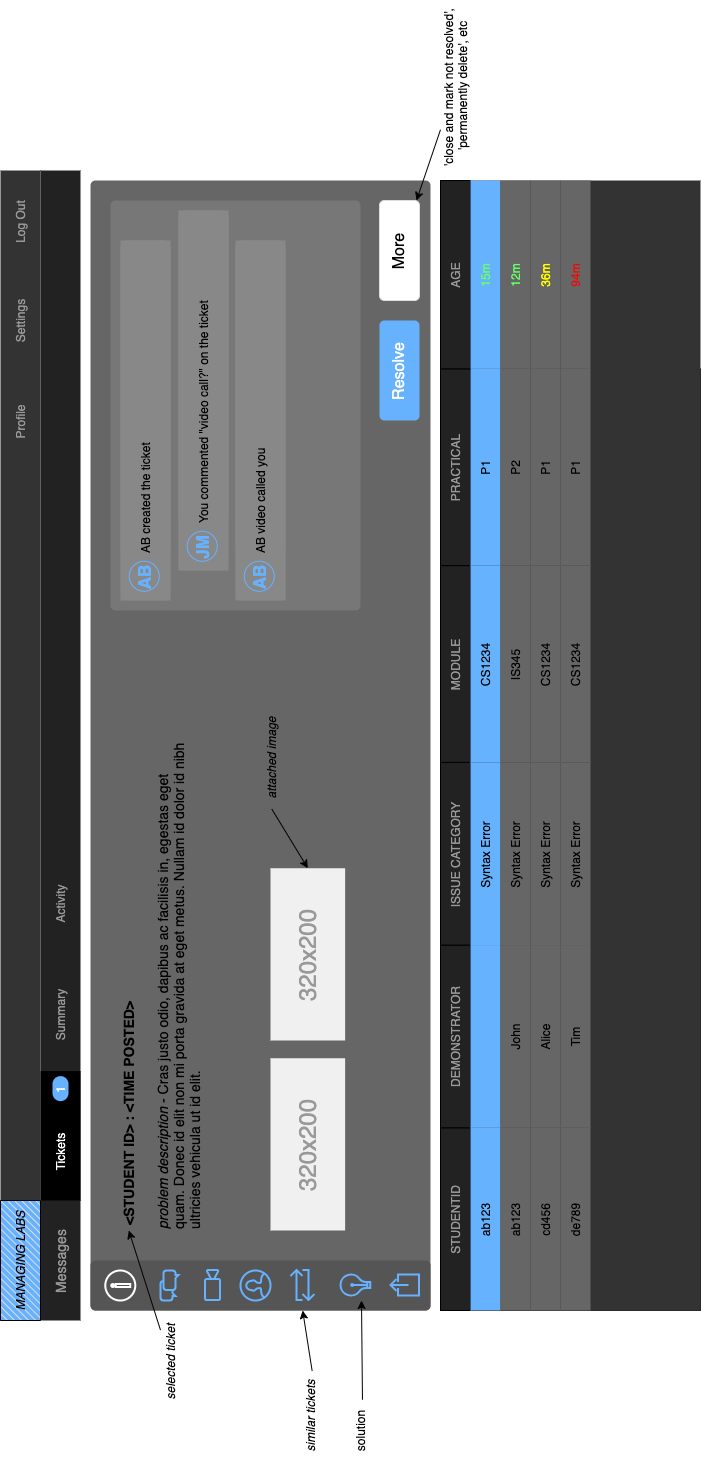
\includegraphics[width=0.6\textwidth]{7design/images/demoTickets.png}
    \caption{Simple design for the demo ticket viewing interface.}
    \label{fig:demoTickets}
\end{figure}

\section{Database}

\subsection{Entities, Attributes and Relationships}
We will now define a representation of the data in terms of entities, attributes and relationships between entities.

\subsubsection{Entities}

We represent the components of the systems as the following entities. 

\FloatBarrier
\begin{table}[H]
\centering
\begin{tabular}{ |l|c| } 
 \hline
 \textbf{Entity Set} & \textbf{Attributes}\\ 
 \hline
  user & \underline{username}, name\\ 
 \hspace{6pt}user.student & \\ 
 \hspace{6pt}user.demonstrator & \\
 \hspace{12pt}user.demonstrator.labLead & \\
 auth & \underline{username}, password, role \\
 ticket & \underline{ticketId}, issueDescription,\\
 & practical, resolutionStatus \\
 attachment & \underline{attachmentId}, file, caption \\
 lab & \underline{labId}, openTime, closeTime\\
 solution & \underline{solutionId}, solutionDescription\\
 category & \underline{name} \\
 module & \underline{moduleCode} \\
 \hline
\end{tabular}
\caption{Table of entities and associated attributes.}
\end{table}
\FloatBarrier

Primary keys are denoted as \underline{underlined}. Foreign keys are denoted in \textit{italics}.

Note that \textbf{user.student} and \textbf{user.demonstrator} are disjoint specialisations of the entity set \textbf{user} - a user is always a student or demonstrator (or specialisation of demonstrator). \textbf{user.demonstrator.labLead} is a further specialisation of \textbf{user.demonstrator}, not disjoint. 

\subsubsection{Relationships}
We shall now define the relationships between entities and the constraints on them. 

\FloatBarrier
\begin{table}[H]
\centering
\begin{tabular}{ |c|c|c|c| } 
 \hline
 \textbf{Relationship} & \textbf{Entities} & \textbf{Participation} & \textbf{Cardinality}\\ 
 \hline
 $r$ & $e_1$, $e_2$ & total, partial & M-1 \\
 \hline
\end{tabular}
\end{table}
\FloatBarrier 

We denote many as M, one as 1 such that one to many relationship would be denoted 1-M. Note that for a relationship $r$ that is many (in $e_1$) to one (in $e_2$) and has total participation from $e_1$ but partial from $e_2$ then the row in the table is written as above. Participation will be listed in order that entities are written.

\FloatBarrier
\begin{table}[htbp]
\centering
\resizebox{\columnwidth}{!}{\begin{tabular}{ |c|c|c|c|c| } 
 \hline
 \textbf{Relationship} & \textbf{Relationship Attributes} & \textbf{Entity Sets} & \textbf{Participation} & \textbf{Cardinality}\\ 
 \hline
 creates & creation\_timestamp & user.student, ticket & partial, total & 1-M \\
 assignedTo & demAssigned\_timestamp & user.demonstrator, ticket & partial, partial & 1-M\\
 writes & demSolved\_timestamp & user.demonstrator, solution & partial, total & M-M\\
 leads & & user.demonstrator.labLead, lab & partial, total & 1-M\\
 hasAttachment & ticket\_attach\_timestamp & ticket, attachment & partial, partial & 1-M\\
 hasAttachment & solution\_attach\_timestamp & solution, attachment & partial, partial & 1-M\\
 postedIn &  & ticket, lab & total, partial & M-1\\
 hasTicketCat & & ticket, category & total, partial & M-M\\
 hasSolutionCat & & solution, category & total, partial & M-M\\
 demonstratesInLab& & user.demonstrator, lab & partial, total & M-M\\
 enrolledInMod && user.student, module & total, partial & M-M\\
 demonstratesInMod && user.demonstrator, module & partial, partial & M-M\\
 leadsMod && user.ladLead, module & partial, partial & 1-M\\
 toDoWith && ticket, module & total, partial & M-1\\
 hasAuth && user, auth & total, total & 1-1 \\ 
 \hline
\end{tabular}}
\caption{Table showing entities, relationships between, relationship attributes, participation and cardinality.}
\end{table}
\FloatBarrier

\subsubsection{Entity Relationship Diagram}

\begin{figure}[H]
    \centering
    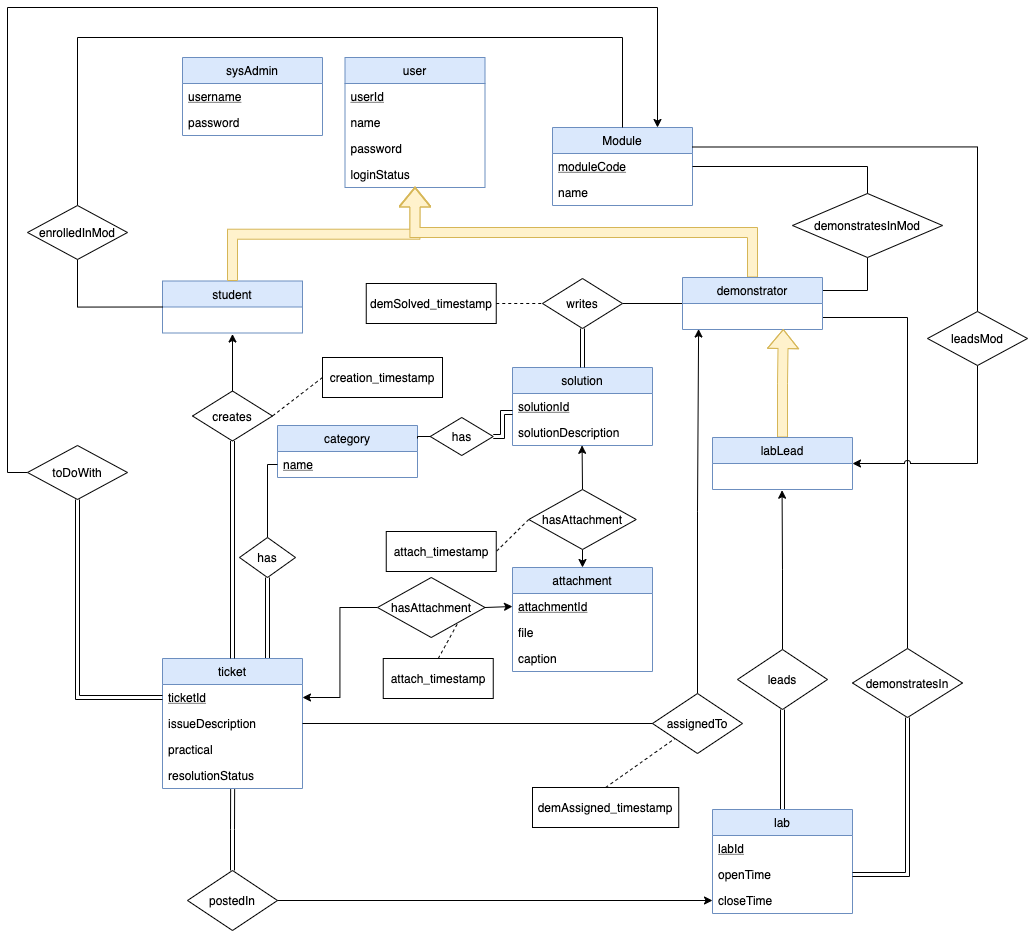
\includegraphics[width=\textwidth]{7design/images/ER.png}
    \caption{\gls{er} diagram for the system.}
    \label{fig:ER}
\end{figure}

\subsubsection{Relational Schema}
The first task is to translate the given E-R model into corresponding database schema below.\\

\noindent student - \underline{\textit{username}}, name, enrolledModules \\
demonstrator - \underline{\textit{username}}, name, demonstratedModules \\
labLead - \underline{\textit{username}}, name, demonstratedModules, ledModules \\
auth - \underline{username}, password, role \\
ticket - \underline{ticketId}, issueDescription, module, practical, resolutionStatus, \textit{student.username}, creation\_timestamp, \textit{demonstrator.username}, demAssigned\_timestamp, \textit{labId} \\
category - \underline{name} \\
solution - \underline{solutionId}, solutionDescription\\
attachment - \underline{attachmentId}, file, caption, \textit{ticketId}, ticket\_attach\_timestamp, \textit{solutionId}, solution\_attach\_timestamp\\
lab - \underline{labId}, title, openTime, closeTime, \textit{labLead.username}\\
writes - \underline{\textit{demonstrator.username}}, \underline{\textit{solutionId}}, demSolved\_timestamp\\
hasTicketCat - \underline{\textit{tickedId}}, \underline{\textit{name}}\\
hasSolutionCat - \underline{\textit{solutionId}}, \underline{\textit{name}}\\
demonstratesInLab- \underline{\textit{demonstrator.username}}, \underline{\textit{labId}}\\
module - \underline{moduleCode}, name, \textit{labLead.username}\\
enrolledInMod - \underline{\textit{student.username}}, \underline{\textit{moduleCode}}\\
demonstratesInMod - \underline{\textit{demonstrator.username}}, \underline{\textit{moduleCode}}\\

\subsubsection{Relational Schema Diagram}

\begin{figure}[H]
    \centering
    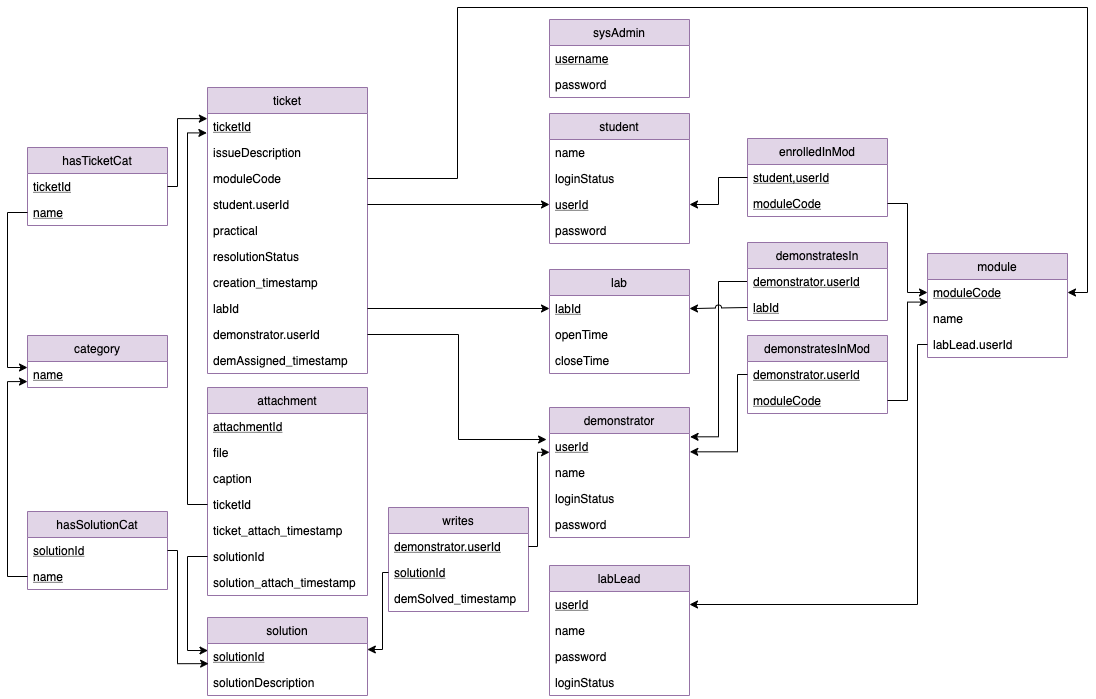
\includegraphics[width=0.8\textwidth]{7design/images/relationalSchema.png}
    \caption{Relational schema diagram for the system.}
    \label{fig:relationalschema}
\end{figure}

\subsubsection{Attribute Types}
A data type must be specified for each attribute. Table \ref{table:atypetable} below shows the attribute type for each attribute, as well as it's original, parent relational table - in other words, we do not repeat the attributes that appear as foreign keys in tables.

\begin{table}[H]
\centering
\begin{tabular}{| c | c | c | c |}
\hline
 Relational Table & Attribute & Attribute Type & Notes\\ 
 \hline
  category & name & VARCHAR(70) & Government data standards\cite{dataStandards}\\
  \hline
  ticket & ticketId & INT & Auto incremented by DB.\\
  & issueDescription & VARCHAR(2000)&\\
  & practical & VARCHAR(6)&preset list?\\
  & resolutionStatus & VARCHAR(8)&[new, missed, inProgress, closed]\\
  & creation\_timestamp & DATE &\\
  &  demAssigned\_timestamp & DATE &\\
  \hline 
  attachment & attachmentId & INT & Auto incremented by DB.\\
  & file & BLOB &\\
  & caption & VARCHAR(150) & \\
  & ticket\_attach\_timestamp & DATE &\\
  & solution\_attach\_timestamp & DATE& \\
  \hline
  solution & solutionId & INT&Auto incremented by DB.\\
  & solutionDescription & VARCHAR(2000)&\\
  \hline
  writes & demSolved\_timestamp & DATE &\\
  \hline
  sysAdmin & username & VARCHAR(16) &\\
  & password & CHAR(60) & hashed password\\
  \hline
  student & name & VARCHAR(70) & Government data standards\cite{dataStandards}\\
  & username & INT&studentnumber details?\\
  & password & CHAR(60)&hashed password\\
  \hline
  lab & labId & INT&Auto incremented by DB.\\
  & title & VARCHAR(70) & \\
  & openTime & DATE &\\
  & closeTime & DATE &\\
  \hline
  demonstrator & username & VARCHAR(16)&\\
  & name & VARCHAR(70)& Government data standards\cite{dataStandards}\\
  & password & CHAR(60) &hashed password\\
  \hline
  labLead & username & VARCHAR(16)&\\
  & name & VARCHAR(70) & Government data standards\cite{dataStandards}\\
  & password & CHAR(60)& hashed password\\
  \hline
  module & moduleCode & CHAR(6) & Fixed type [A-Z]\{2\}\arraybackslash \textbackslash d\{4\}
\\
  & name & VARCHAR(70)& Government data standards\cite{dataStandards}\\
 \hline
 
 \hline
\end{tabular}
\caption{Table describing the data types for attributes, showing the parent relational table.}
\label{table:atypetable}
\end{table}

The Government Data Standards Catalogue\cite{dataStandards} was referenced for the data types corresponding to names - including logical extension to category and module names. 

ID data types are defined as INT,auto increment from db. 

\subsection{choices}

-react / enterprise level -> load balancing
-why sql
-data access object